\documentclass[../../../patent_v1.tex]{subfiles}

\begin{document}

From the abstract, we can conclude that speaker angles and sound intensities of 
individual speakers are essential.

Speaker angles define how the sound is going to reach the listener. Like is it 
reflecting from any surface, or the sound sources are directly pointed towards the 
listener.

Sound is nothing but oscillations of particles (typically air) in vibrational motion, 
which transports energy through a medium.

\begin{figure}
    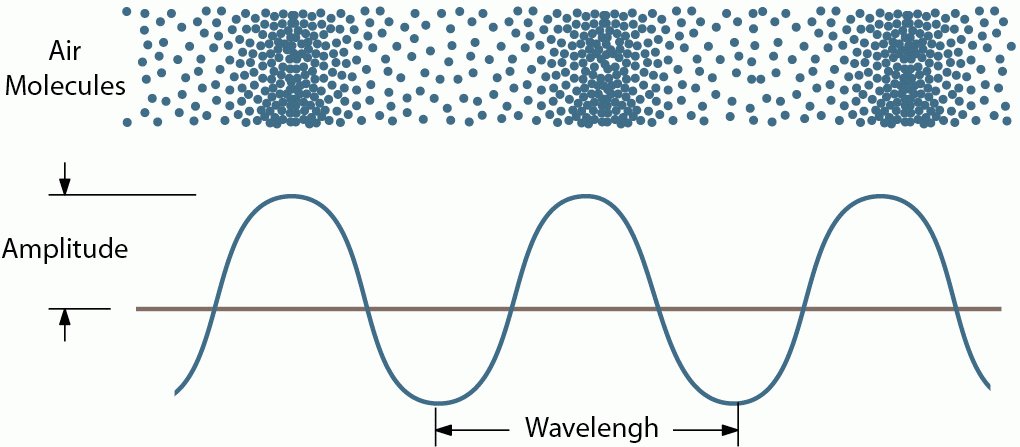
\includegraphics[width=\columnwidth]{sound_waves.png}
    \caption{Sound Waves}
\end{figure}

\FloatBarrier

Speakers push and pull surround air molecules in waves to generate a sound wave using a 
diaphragm. Typically, this diaphragm is in conical shape; hence it oscillates the 
molecules in the oval field. 

\begin{figure*}[ht]
    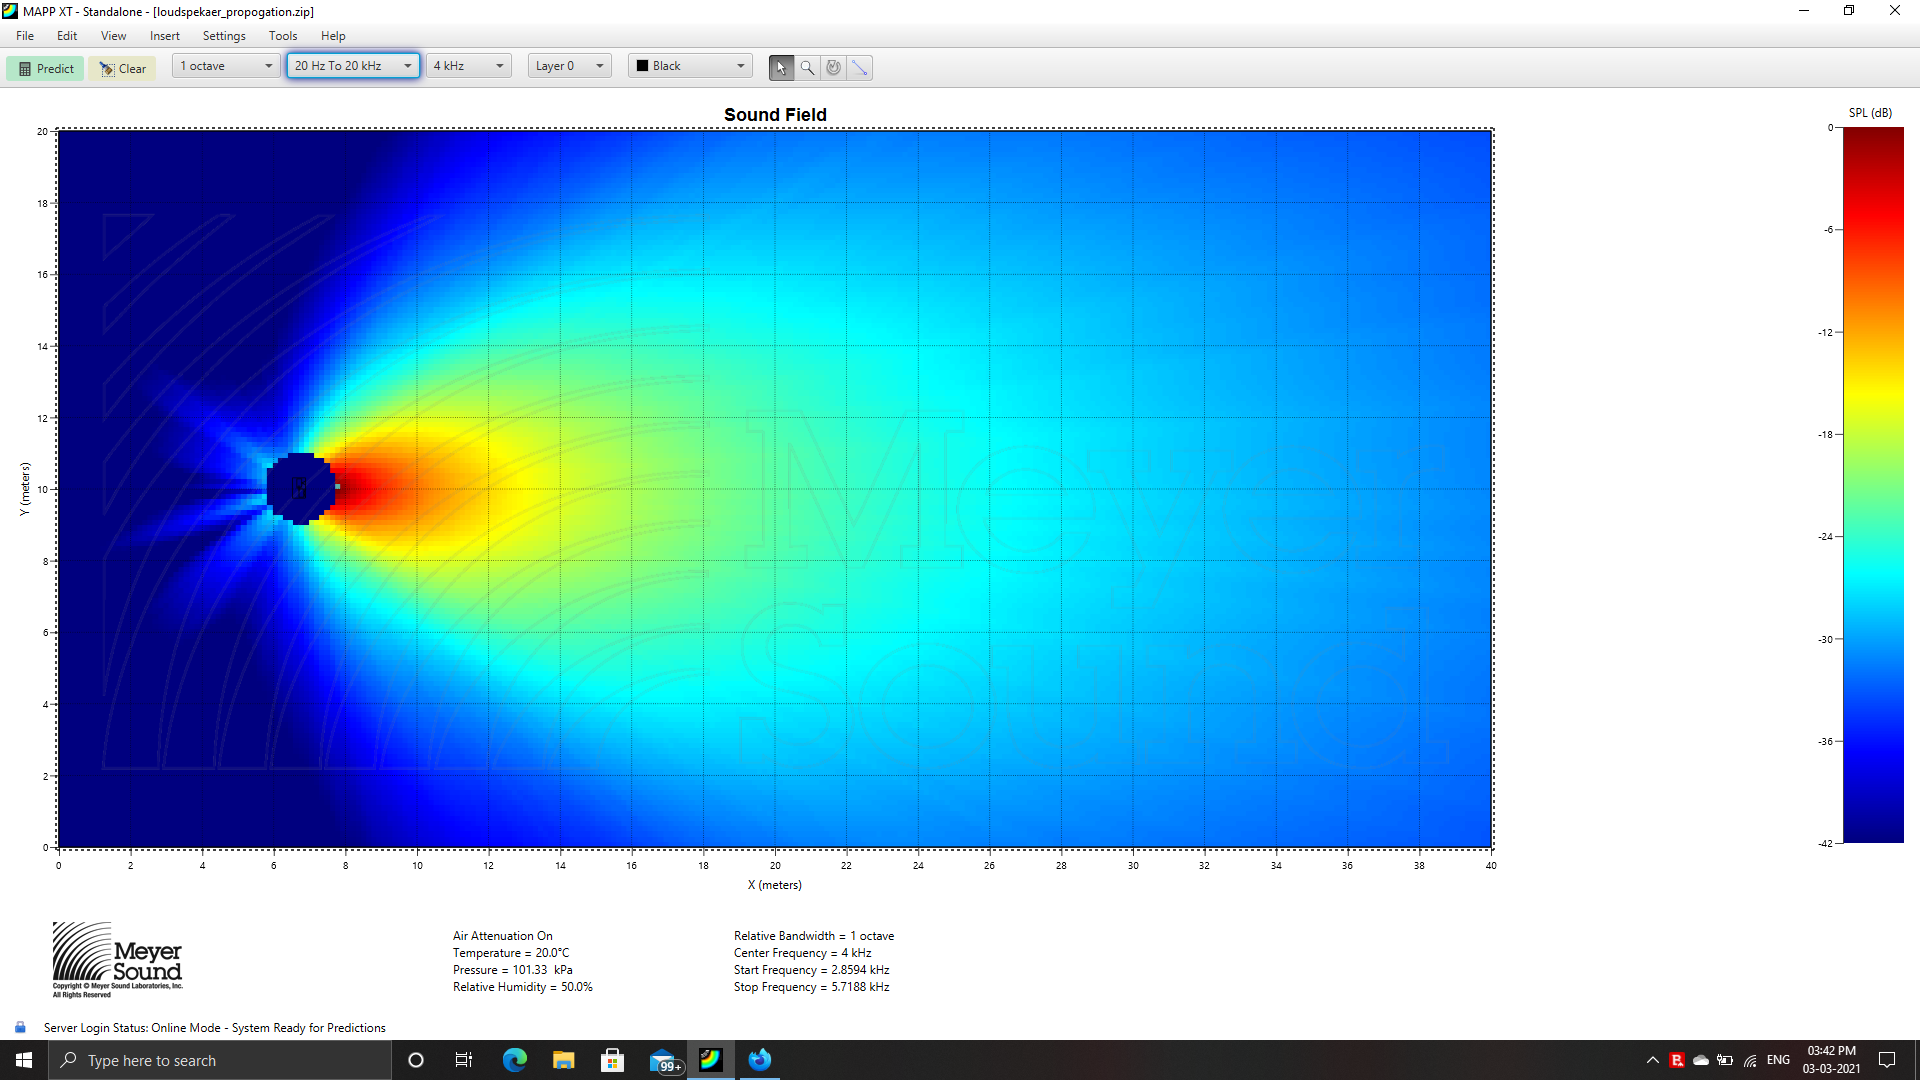
\includegraphics[width=1\textwidth]{sound_propogation_for_speaker.png}
    \caption{Sound propagation of a speaker}
\end{figure*}

\FloatBarrier

Figure 3.2 shows the oval propagation of the sound field from the speaker. The speaker's 
sound intensity at some depth is denoted with a heat map (dB). In front of the speaker, 
the sound intensity is maximum, and it fades away as we go far away from the speaker. 
Where, on the other hand, it is much less at the back of the speaker. Since it is oval, 
the propagation to left and right is also less than that of the front.

Figure 3.3 shows the reflection and reverberation of sound due to misalignment and the 
speaker's excessive sound intensity due to the collision of sound waves onto walls. 
These reverberations decay as they get absorbed by the surfaces of objects and walls in 
the room. In this case, the listener tends to hear the direct and repeated sound waves, 
which might sound muddy and grabbled.

\begin{figure}
    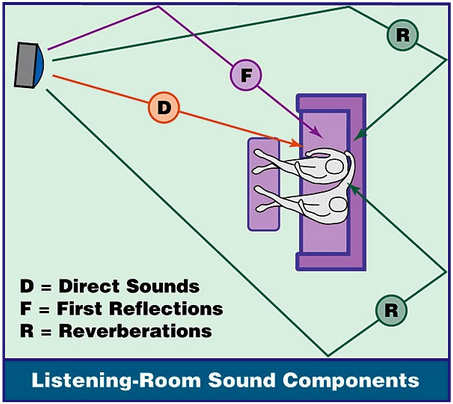
\includegraphics[width=\columnwidth]{reverberation.png}
    \caption{Reflection and reverberation of sound}
\end{figure}

\FloatBarrier

Hence, it becomes necessary to align the speakers and adjust the sound levels in proper 
amounts to get the best surround sound.

To overcome this scenario, we experimented with a five-block system. 
Which consists of,

\begin{description}
    \item[1.]Depth estimation unit (Cameras), to measure the listener's depth from one 
    reference point and feed these variables to the microprocessor for further 
    calculations.
    \item[2.]Microprocessor, to measure depth and calculate 
    panning and tilting angles and listener's depth
    from each speaker.
    \item[3.]Mechanical unit, to pan and tilt the speakers.
    \item[4.]Audio Processor Unit (Digitally controlled amplifier) adjusts the individual 
    speaker gain using calculated results from the microprocessor.
    \item[5.]Speakers, to sound individual 4-channeled output.
\end{description} 

\end{document}